\documentclass{standalone}
\usepackage{tikz}
\begin{document}
% TI-84 Plus CE list editor (STAT > EDIT); 1 unit = 1 screen pixel of the 244x184 screenshot
\newcommand{\Ls}[1]{L\raisebox{-0.35ex}{\fontsize{5}{5}\selectfont #1}}
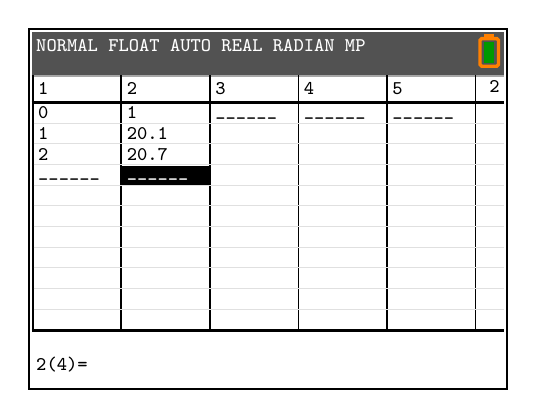
\begin{tikzpicture}[x=0.025cm, y=-0.025cm,
    every node/.style={inner sep=0pt, font=\ttfamily\bfseries\fontsize{7}{8}\selectfont}]
  % Screen background and border
  \fill[white] (0,0) rectangle (244,184);
  % Status bar
  \fill[black!68] (2,2) rectangle (242,24);
  \node[anchor=west, text=white] at (4,9) {NORMAL FLOAT AUTO REAL RADIAN MP};
  % Battery icon (full)
  \draw[orange, line width=1.2pt, rounded corners=0.6pt] (229.8,5.5) rectangle (239.2,19.5);
  \fill[orange] (232,3) rectangle (237,5);
  \fill[green!60!black] (232,7) rectangle (237,18);
  % Table frame: header underline (thick), column dividers, bottom line
  \draw[black!35, line width=0.4pt] (2,24.5) -- (242,24.5);
  \draw[black, line width=1.2pt] (2,38) -- (242,38);
  \foreach \x in {2,47,92,137,182,227}
    \draw[black, line width=0.6pt] (\x+0.5,24) -- (\x+0.5,154);
  \draw[black, line width=1pt] (2,154) -- (242,154);
  % Faint row separators
  \foreach \y in {48.5,59,69.5,80,90.5,101,111.5,122,132.5,143}
    \draw[black!12, line width=0.3pt] (3,\y) -- (242,\y);
  % Column headers
  \node[anchor=west] at (5,31)   {\Ls{1}};
  \node[anchor=west] at (50,31)  {\Ls{2}};
  \node[anchor=west] at (95,31)  {\Ls{3}};
  \node[anchor=west] at (140,31) {\Ls{4}};
  \node[anchor=west] at (185,31) {\Ls{5}};
  \node[anchor=east] at (240,30) {2};
  % L1 data
  \node[anchor=west] at (5,43)   {0};
  \node[anchor=west] at (5,54)   {1};
  \node[anchor=west] at (5,64.5) {2};
  \node[anchor=west] at (5,77.5) {------};
  % L2 data, with cursor highlighting the empty 4th entry
  \node[anchor=west] at (50,43)   {1};
  \node[anchor=west] at (50,54)   {20.1};
  \node[anchor=west] at (50,64.5) {20.7};
  \fill[black] (48,70) rectangle (92,80);
  \node[anchor=west, text=white] at (50,77.5) {------};
  % L3, L4, L5 empty
  \foreach \x in {95,140,185}
    \node[anchor=west] at (\x,46.5) {------};
  % Entry line
  \node[anchor=west] at (4,171) {\Ls{2}(4)=};
  % Outer screen border
  \draw[black, line width=0.8pt] (0.5,0.5) rectangle (243.5,183.5);
\end{tikzpicture}
\end{document}
